\newpage
\section*{Pruebas unitarias}
\subsection*{Smart Owl}
\begin{center}
  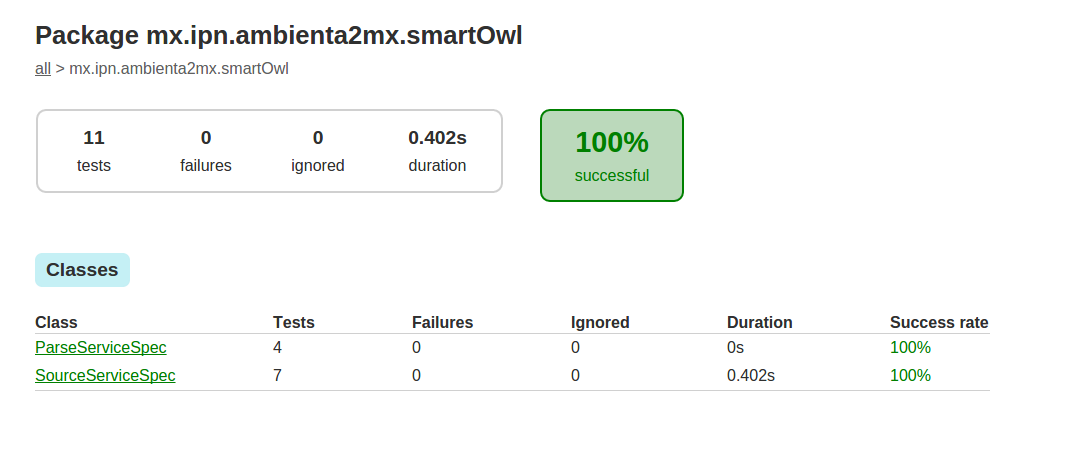
\includegraphics[width=\textwidth]{images/SmartOwlTest1}
\end{center}

\begin{center}
  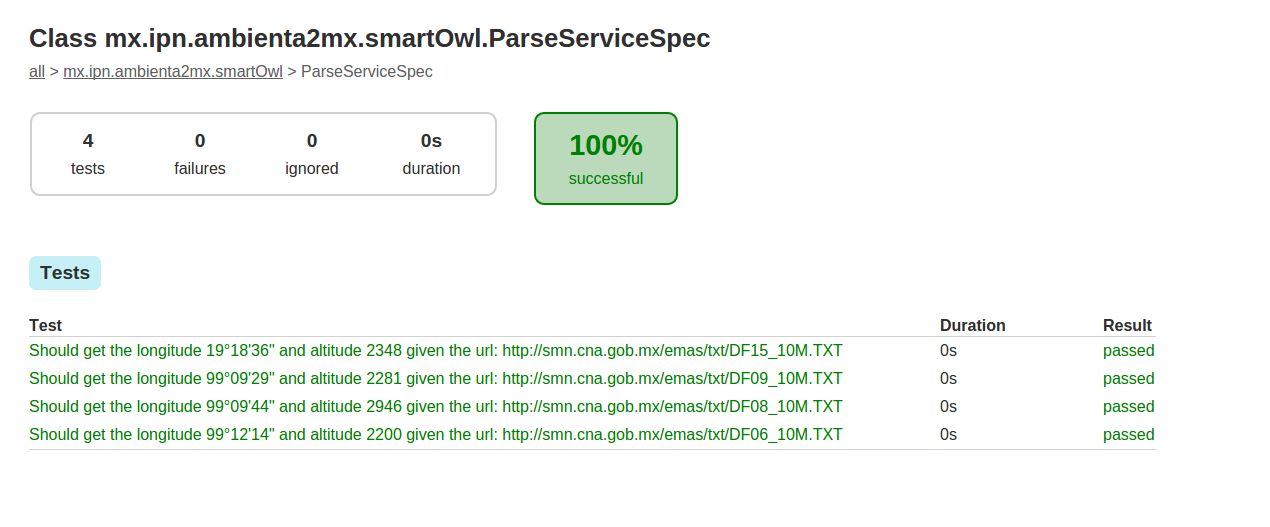
\includegraphics[width=\textwidth]{images/SmartOwlTest2}
\end{center}

\begin{center}
  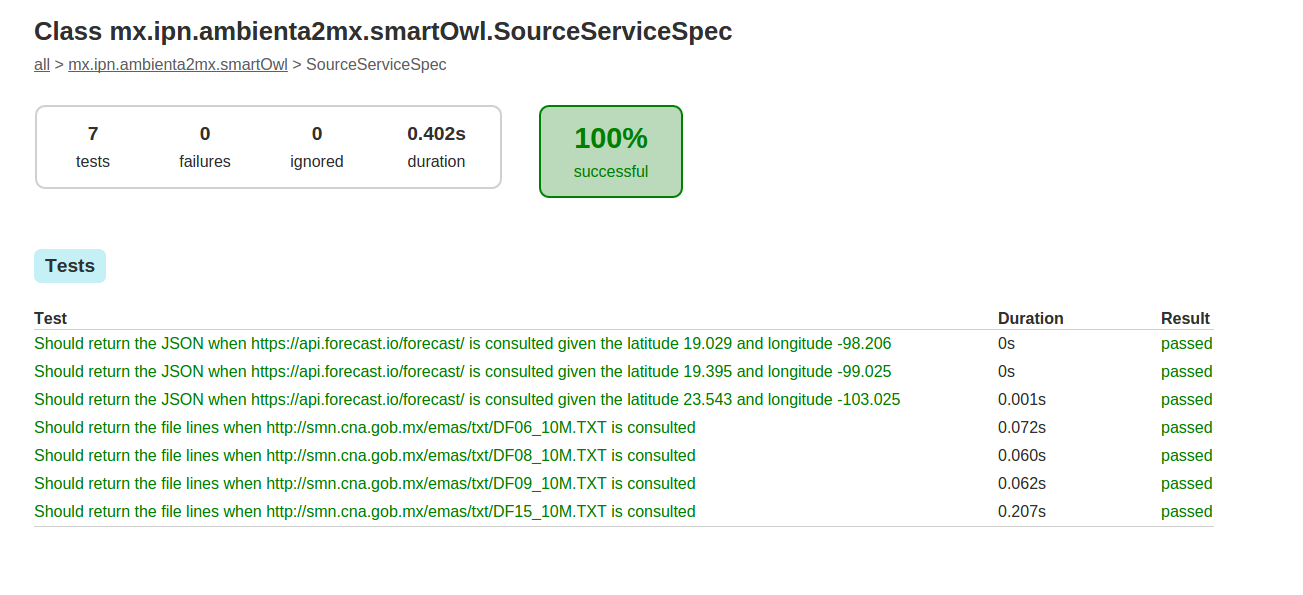
\includegraphics[width=\textwidth]{images/SmartOwlTest3}
\end{center}
\addcontentsline{toc}{chapter}{Anexo 1: Pruebas Unitarias}
%
% User stories
%
\newpage
\section*{Historias de Usuario}
\subsection*{Friendly Dolphin}
  \begin{itemize}
    \item US1 Reporte de información climática actual
    \begin{itemize}
      \item \textbf{Como} usuario de Friendly Dolphin
      \item \textbf{Quiero} consultar la información climática actual
      \item \textbf{De tal manera} que pueda generar un reporte con la información estandarizada.
    \end{itemize}
    \item Criterios de Aceptación
    \begin{itemize}
      \item Seleccionar una región del pais.
      \item Se deberá mostrar la información en texto plano.
      \item Opción para exportar la información en formato JSON o XML.
    \end{itemize}
  \end{itemize}
  \begin{itemize}
    \item US2 Historial de información climática
    \begin{itemize}
      \item \textbf{Como} usuario de Friendly Dolphin
      \item \textbf{Quiero} consultar el historial de los datos climáticos.
      \item \textbf{De tal manera} que pueda visualizar de manera gráfica el cambio de los valores de las variables climáticas a través de un periodo de tiempo
    \end{itemize}
    \item Criterios de Aceptación
    \begin{itemize}
      \item Consultar la información entre una fecha de Inicio y una fecha Final.
      \item Se deberá mostrar la información de las variables climáticas en el periodo seleccionado.
      \item Opción para exportar la información en formato JSON o XML.
    \end{itemize}
  \end{itemize}
\addcontentsline{toc}{chapter}{Anexo 2: Historias de Usuario.}
%
% RESTful Services
%
\newpage
\section*{Servicios REST}
\paragraph{La ventaja al usar servicios de tipo REST, es la sencillez al cambiar el contenido que se expone sin tener que cambiar o generar un protocolo de comunicación ya que toma como base HTTP}.
\paragraph{Simplemente es necesario con un cliente, desde un navegador web hasta clientes dedicados a servicios REST, para poder accedera a los recursos expuestos. Todas las API's rest siguen una convención de verbos tomados de la base de HTTP (GET, POST, PUT, DELETE).}
\paragraph{En comparación con servicios de tipo SOAP, no se requiere una alta atomicidad y ni transacciones, una de las razones por la que los servicios WS suelen ser usados.}
\paragraph{Finalmente, los servicios de tipo REST pueden tener respuestas en diversos formatos, principalmente JSON y XML, esto brinda al desarollador o a la persona que consula como tratar la respuesta por bibliotecas de terceros o nativas.}
\paragraph{El soporte para formatos JSON es nativo en los navegadores web, otra de las razones por las cuales éstos servicios han ido ganando mercado ya que el desarrollo de aplicaciones Web ha aumentado de forma drástica en los últimos años. \cite{31}}
\addcontentsline{toc}{chapter}{Anexo 3: Servicios REST}